\section{Non local Maxwell Condition}



We are seeking an analog of the Maxwell condition for the bleb model, and similar non-local PDEs. We will make progress toward on this by studying the following systems, from most general (Equations ~\ref{eq::gensystema},~\ref{eq::gensystemy})  to most the most narrow (Equations ~\ref{eq::a_ODE}, ~\ref{eq::gen_ym}).  In the fast timescale, we have $c = c^{ss}$.  The dynamics of excitation are thus only governed by the $a$ equation. We are ultimately interested in a necessary and sufficient traveling wave condition for the general system

\begin{align}
\dfrac{\partial a}{ \partial t}  & =  f(a,y)\label{eq::gensystema}\\
0 & =g \left(a,y,\dfrac{\partial^2 y}{\partial x^2}\right). \label{eq::gensystemy}
\end{align}
Our specific system restricted to the fast timescale is
\begin{align}
\dfrac{\partial a}{ \partial t}  & =  \dfrac{c^{ss}}{1+c^{ss}} \mbox{exp}\left(-\dfrac{y-y_C}{D}\right) - a \mbox{exp} \left(\dfrac{y-y_C}{F} \right)\label{eq::a_ODE}\\
0 & = -a(y - y_C) + P (1-y) + \gamma_M \dfrac{\partial^2 y}{\partial x^2}\label{eq::yM_eq} \\
0 & = a(y-y_C) - Mcy_C\label{eq::nondimyC2}.
\end{align} 
Note that since Eq.~\ref{eq::nondimyC2} is algebraic in $y_C$, we can eliminate it from the system. A narrow version of the system is obtained if we assume the force balance equations are linear in $a$.

\begin{align}
\dfrac{da}{ dt}  & = f_1(y) - a f_2(y)\label{eq::gen_a}\\
0 & = g_1(y) - ag_2(y) +  \dfrac{\partial^2 y}{\partial x^2}\label{eq::gen_ym}
\end{align}
This can be obtained from our system given the following simplifying assumption. Assume that the variable, $y_C$ does not move significantly during excitation, $y_C = y_C^{ss}$, leaving us with the new system of two equations:
\begin{align}
\dfrac{\partial a}{ \partial t}  & =  \dfrac{c^{ss}}{1+c^{ss}} \mbox{exp}\left(-\dfrac{y-y_C^{ss}}{D}\right) - a \mbox{exp} \left(\dfrac{y-y_C^{ss}}{F} \right)\label{eq::a_ODE}\\
0 & = -a(y - y_C^{ss}) + P (1-y) + \gamma_M \dfrac{\partial^2 y}{\partial x^2}\label{eq::yM_eq}
\end{align} 
We derive a necessary condition for the system described by Equations ~\ref{eq::a_ODE} and ~\ref{eq::gen_ym} here. 

\subsection{Numerical observation of travelling waves} Numerically, we observe a travelling wave solution  to the system described by (D) and is shown in Fig.~\ref{fig::A_wave}.
\begin{figure}[h]
\centering
\captionsetup{width=.9\linewidth}
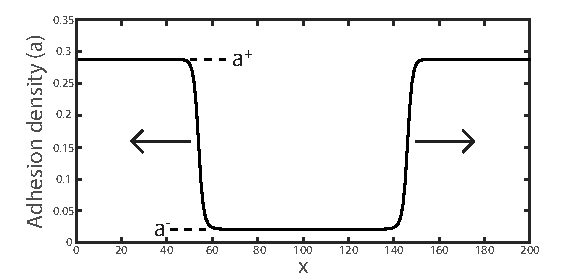
\includegraphics[width=4.5in]{Project2/figs/A_wave.pdf}
\caption{Snapshot of the travelling wave from simulation of Eq.~\ref{eq::a_ODE} and~\ref{eq::yM_eq}.}
\label{fig::A_wave}
\end{figure}

\subsection{Transformation to $z$ coordinate and derivation of non-local Maxwell condition} 
We assume, WLOG, that Eq.~\ref{eq::gen_a} has two stable roots which we will denote by $(y^{+},a^{+})$ and $ (y^{-},a^{-})$.
Transform to wave coordinate $z = x-vt$ and~\ref{eq::gen_a} and~\ref{eq::gen_ym} become:
\begin{align}
-v \dfrac{da}{ dz}  & = f_1(y) - a f_2(y)\label{eq::gen_a_z}\\
0 & = g_1(y) - ag_2(y) +  \dfrac{\partial^2 y}{\partial z^2}\label{eq::gen_ym_z}
\end{align}
We can use Eq.~\ref{eq::gen_ym_z} to solve for $a$:
\begin{flalign}
 a = \dfrac{1}{g_2(y)} \left( g_1(y) + \dfrac{\partial^2 y}{\partial z^2} \right)
\end{flalign}
Then it follows that:
\begin{equation}\Rightarrow  -v \dfrac{\partial a}{ \partial z}   =  f_1(y)  -  \dfrac{g_1(y)}{g_2(y)}f_2(y) - \dfrac{f_2(y)}{g_2(y)} \dfrac{\partial^2 y}{\partial z^2}
\end{equation}
Multiply by $ \dfrac{g_2(y)}{f_2(y)} $,
\begin{equation}\Rightarrow   -v \dfrac{\partial a}{ \partial z} \dfrac{g_2(y)}{f_2(y)}   =  f_1(y)\dfrac{g_2(y)}{f_2(y)}  -  g_1(y) -  \dfrac{\partial^2 y}{\partial z^2}
\end{equation}
Multiply by $\dfrac{\partial y}{\partial z}$,
\begin{equation}\Rightarrow  -v \dfrac{\partial a}{ \partial z} \dfrac{g_2(y)}{f_2(y)} \dfrac{\partial y}{\partial z}   =  \left( f_1(y)\dfrac{g_2(y)}{f_2(y)}  -  g_1(y) -  \dfrac{\partial^2 y}{\partial z^2} \right)  \dfrac{\partial y}{\partial z}
\end{equation}
Integrate over $z$, 
\begin{equation}
\Rightarrow  \int_ {- \infty}^{\infty}  -v \dfrac{\partial a}{ \partial z} \dfrac{g_2(y)}{f_2(y)} \dfrac{\partial y}{\partial z} dz = \int_ {- \infty}^{\infty} \left( f_1(y)\dfrac{g_2(y)}{f_2(y)}  -  g_1(y) -  \dfrac{\partial^2 y}{\partial z^2} \right)  \dfrac{\partial y}{\partial z} dz
\end{equation}
Change variables on RHS,   
\begin{align}\Rightarrow -v  \int_ {- \infty}^{\infty}  \dfrac{\partial a}{ \partial z} \dfrac{g_2(y)}{f_2(y)} \dfrac{\partial y}{\partial z} dz &= \int_ {y^{-}}^{y^{+}} \left( f_1(y)\dfrac{g_2(y)}{f_2(y)}  -  g_1(y) -  \dfrac{\partial^2 y}{\partial z^2} \right)  dy \\
\Rightarrow  -v  \int_ {- \infty}^{\infty}  \dfrac{\partial a}{ \partial z} \dfrac{g_2(y)}{f_2(y)} \dfrac{\partial y}{\partial z} dz &= \int_ {y^{-}}^{y^{+}} \left( f_1(y)\dfrac{g_2(y)}{f_2(y)}  -  g_1(y)\right) dy -  \cancelto{0}{\int_ {y^{-}}^{y^{+}}  \dfrac{\partial^2 y}{\partial z^2}   dy}\\
\Rightarrow -v  \int_ {- \infty}^{\infty}  \dfrac{\partial a}{ \partial z} \dfrac{g_2(y)}{f_2(y)} \dfrac{\partial y}{\partial z} dz &= \int_ {y^{-}}^{y^{+}} \left( f_1(y)\dfrac{g_2(y)}{f_2(y)}  -  g_1(y)\right) dy 
\end{align}
The Non-local Maxwell Condition Number is defined by the RHS of the above equation. In our specific case,
\begin{align}
f_1(y) &=  \dfrac{c^{ss}}{1+c^{ss}} \mbox{exp}\left(-\dfrac{y-y_C^{ss}}{D}\right),\\
f_2(y) &= \mbox{exp} \left(\dfrac{y-y_C^{ss}}{F} \right),\\
g_1(y) &=  P (1-y), \\
 g_2(y) &= (y - y_C^{ss}).
\end{align}
Therefore, 
\begin{multline}
-v  \int_ {- \infty}^{\infty}  \dfrac{\partial a}{ \partial z} \dfrac{(y - y_C^{ss})}{ \mbox{exp} \left(\dfrac{y-y_C^{ss}}{F} \right)} \dfrac{\partial y}{\partial z} dz \\
= \int_ {y^{-}}^{y^{+}} \left( \dfrac{c^{ss}}{1+c^{ss}} \mbox{exp}\left(-\dfrac{y-y_C^{ss}}{D}\right) \dfrac{(y - y_C^{ss})}{ \mbox{exp} \left(\dfrac{y-y_C^{ss}}{F} \right)}  -   P (1-y) \right) dy
\end{multline}
\begin{multline}
\implies -v  \int_ {- \infty}^{\infty}  \dfrac{\partial a}{ \partial z}\dfrac{\partial y}{\partial z} \mbox{exp} \left(-\dfrac{y-y_C^{ss}}{F} \right)(y - y_C^{ss}) dz\\
= \int_ {y^{-}}^{y^{+}}  \left( \dfrac{c^{ss}}{1+c^{ss}} \mbox{exp}\left( -\left( \dfrac{1}{D} + \dfrac{1}{F} \right) (y-y_C^{ss})\right)  -   P (1-y) \right) dy\\
\end{multline}
We also note that in our specific case $y^- > y^+$ and so it makes sense to integrate from $y^+$ to $ y^-$.
\begin{align*}
\Rightarrow & -v  \int_ {- \infty}^{\infty}  \dfrac{\partial a}{ \partial z}\dfrac{\partial y}{\partial z} \mbox{exp} \left(-\dfrac{y-y_C^{ss}}{F} \right)(y - y_C^{ss}) dz\\
& \hspace{2cm}= - \int_ {y^{+}}^{y^{-}}  \left( \dfrac{c^{ss}}{1+c^{ss}} \mbox{exp}\left( -\left( \dfrac{1}{D} + \dfrac{1}{F} \right) (y-y_C^{ss})\right)  -   P (1-y) \right) dy
\end{align*}
Our Non-Local Maxwell condition Number is:
\begin{align}
NLMC &= -\int_ {y^{+}}^{y^{-}}  \left( \dfrac{c^{ss}}{1+c^{ss}} \mbox{exp}\left( -\left( \dfrac{1}{D} + \dfrac{1}{F} \right) (y-y_C^{ss})\right)  -   P (1-y) \right) dy \\
 &= \dfrac{c^{ss}}{1+c^{ss}}  \mbox{exp}\left( +\left( \dfrac{1}{D} + \dfrac{1}{F} \right)y_C^{ss}  \right) \left( y^--y^+ \right) + P\left( 1 - \frac{1}{2}\left( \left(y^+\right)^2-\left(y^-\right)^2\right)\right)
\end{align}
The integral on the LHS is of determined sign (-).  Therefore, the Nonlocal Maxwell Condition is:
\begin{align*}
& NLMC >0 \Rightarrow v \text{ exists, travelling solution}\\
& NLMC <0 \Rightarrow v \text{ does not exist, stationary solution}
\end{align*}
Note that only the second line (necessity) is shown here. The first line (sufficiency) is supported by numerical evidence below.

\subsection{Numerical Results}


After we hold $c$ and $y_C$ constant, we end up with a single PDE. Dropping the spatial term, and analyzing the single ODE we find that the ODE is can be monostable low, in which case the only solution is $0$, monostable high, in which case there is a single steady state solution $\ne 0$ or it can be bistable. See Fig.~\ref{fig::phaseline} for a plot of the single ODE in the various regimes. 
\begin{figure}[h]
\centering
\captionsetup{width=0.9\linewidth}
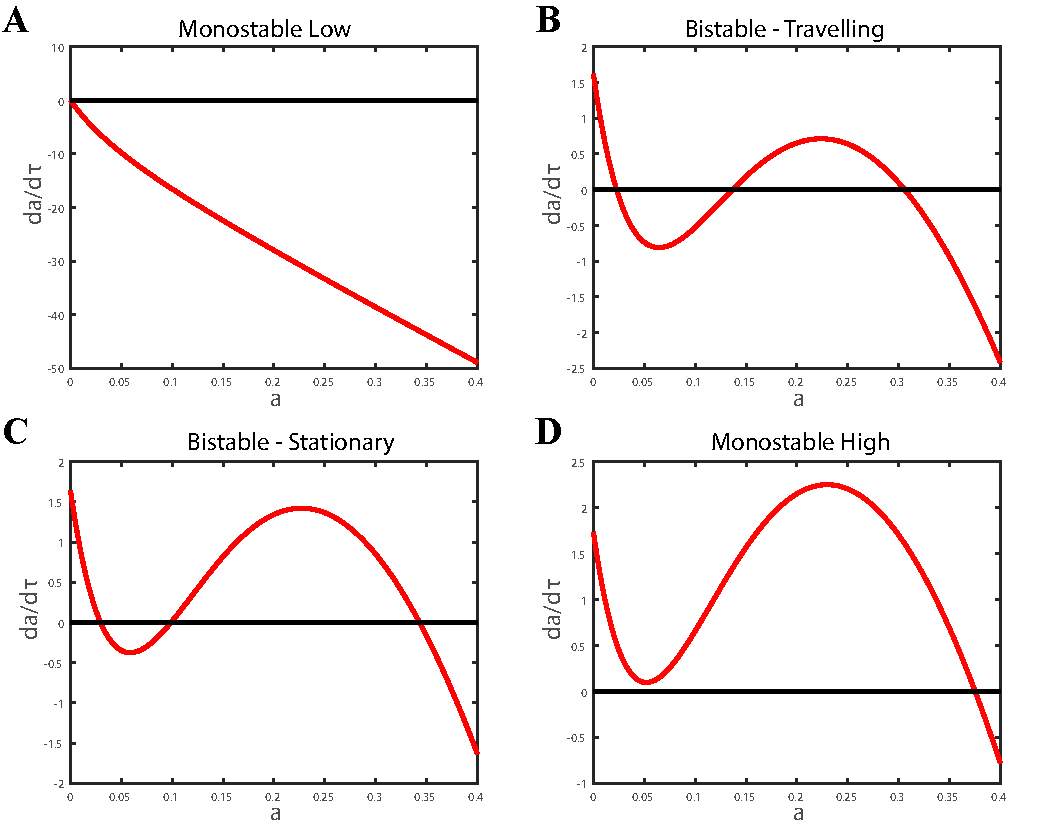
\includegraphics[width=4.5in]{Project2/figs/phaseline.pdf}
\caption{Plot of da/d$t$ vs a for four different parameter sets. A) The monostable zero case, $\Omega = 57$ and $F = 0.95$. B) The bistable ODE-travelling PDE regime, $\Omega = 55$ and $F = 1.2$. C) The  bistable ODE-stationary PDE regime, $\Omega =50 $ and $F = 1.4$. D) The monostable high case,  $\Omega = 45$ and $F = 1.55$.}
\label{fig::phaseline}
\end{figure}

\hspace{6pt}

The non-local Maxwell condition is equal to $0$ in both of the monostable regimes (because $y^- = y^+$), but can be negative or positive in the bistable regime. Returning to the PDE, we don't expect travelling solutions to arise from a monostable regime, but we wish to see for which region of the bistable regime the non-local Maxwell condition predicts travelling solutions. By varying two parameters continuously we can determine these regions. This is shown in Fig.~\ref{fig::NLMC}(A). Here the parameters varied are $\Omega$ which is not present in the single PDE but changes are reflected in $c^{ss}$, and $F$. We plan to create identical plots using other pairs of parameters. The regions shown in Fig.~\ref{fig::NLMC} (A) match up well with the numerical solutions of the PDE as depicted in Eq.~\ref{fig::NLMC} (B), which shows the velocity of the travelling wave solution ($=0$ for a stationary solution).


\begin{figure}[h]
\centering
\captionsetup{width=.9\linewidth}
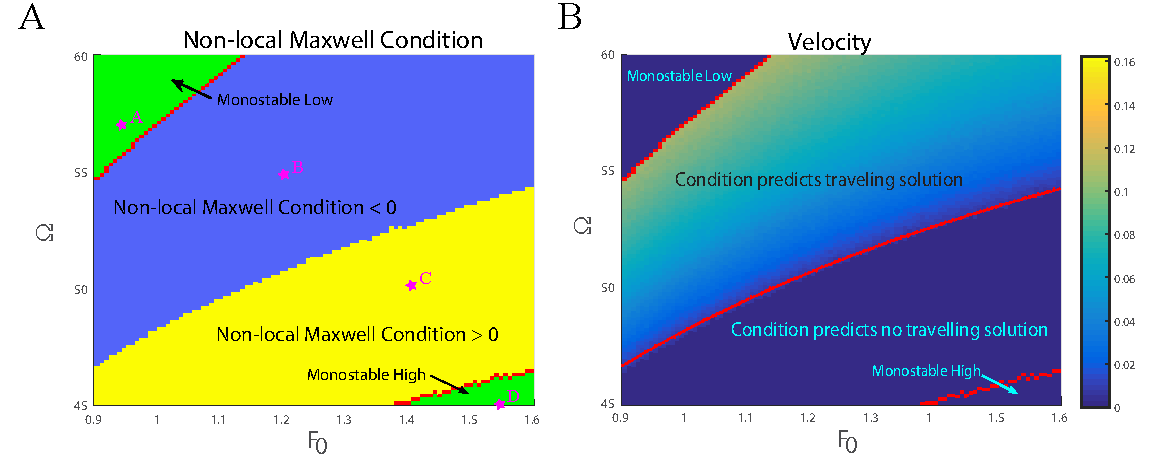
\includegraphics[width=6in]{Project2/figs/MM_results.pdf}
\caption{(A)The results of varying two parameters $\Omega$ and $F$ and the regions where the non-local Maxwell condition is either greater than $0$ (yellow) or less that $0$ (blue). Red lines indicate the boundaries between the monostable and bistable regimes. The pink stars correspond to locations in parameter space where the corresponding phaseline plots of Fig.~\ref{fig::phaseline} were made.  (B) Velocity resulting from numerical solutions of the PDE as two parameters are varied. Red lines indicate the boundaries between the monostable and bistable regimes, as well as the line across which the non-local Maxwell condition is equal to $0$.}
\label{fig::NLMC}
\end{figure}

